\section{Aufbau}
\label{sec:Aufbau}
\begin{figure}
	\centering
	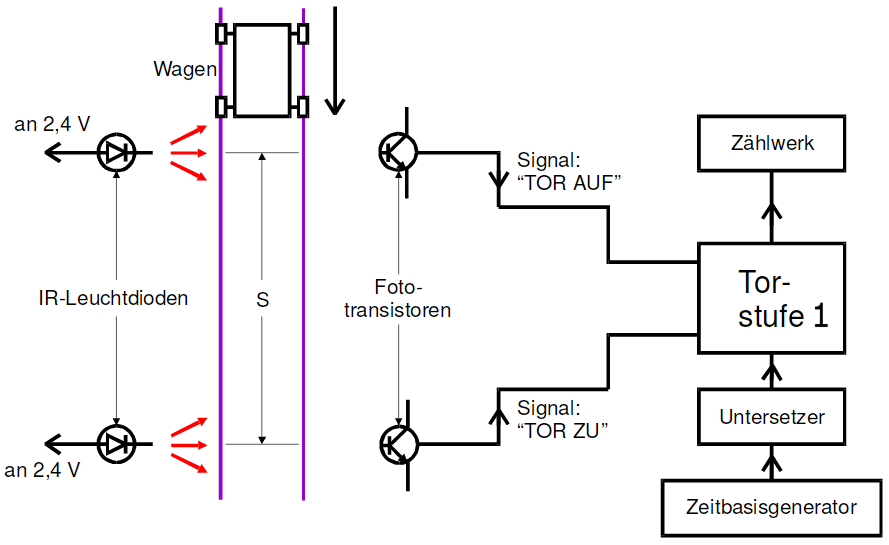
\includegraphics[width=\linewidth-50pt,height=\textheight-50pt,keepaspectratio]{content/Bilder/Geschwindigkeitsmessung.png}
	\caption{Messapperatur zur Geschwindigkeitsbestimmung der einzelnen Motorgänge\cite{V104}.}
	\label{fig:Aufbau}
\end{figure}
\begin{figure}
	\centering
	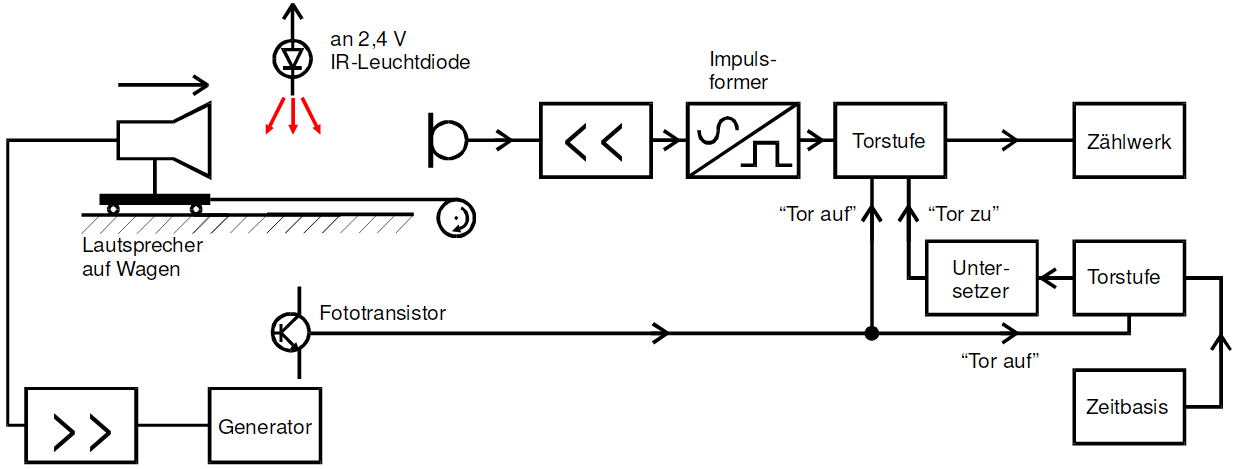
\includegraphics[width=\linewidth-50pt,height=\textheight-50pt,keepaspectratio]{content/Bilder/Frequenzmessung.png}
	\caption{Messapperatur zur Frequenzbestimmung von monofrequenten Schallwellen \cite{V104}.}
	\label{fig:Aufbau}
\end{figure}
\begin{figure}
	\centering
	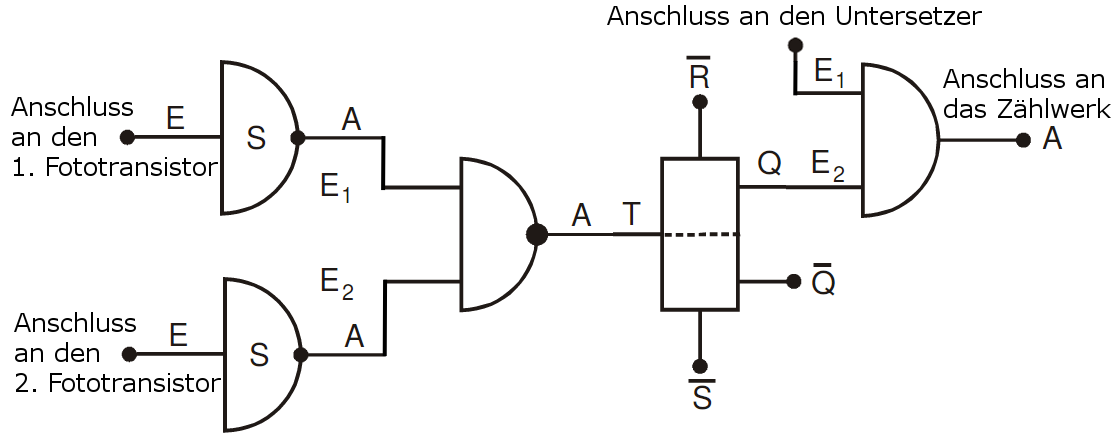
\includegraphics[width=\linewidth-50pt,height=\textheight-50pt,keepaspectratio]{content/Bilder/Torstufe1.png}
	\caption{Torstufe 1 \cite{V104}.}
	\label{fig:Aufbau}
\end{figure}
\begin{figure}
	\centering
	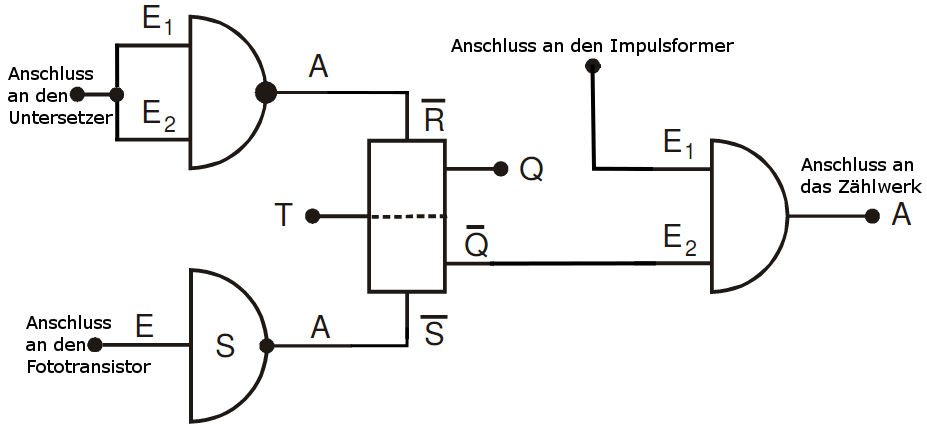
\includegraphics[width=\linewidth-50pt,height=\textheight-50pt,keepaspectratio]{content/Bilder/Torstufe2.png}
	\caption{Torstufe 2 \cite{V104}.}
	\label{fig:Aufbau}
\end{figure}
\begin{figure}
	\centering
	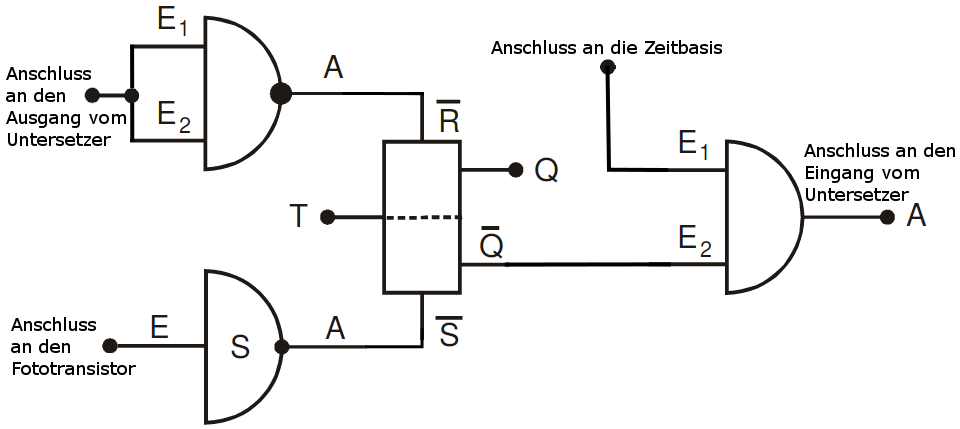
\includegraphics[width=\linewidth-50pt,height=\textheight-50pt,keepaspectratio]{content/Bilder/Torstufe3.png}
	\caption{Torstufe 3 \cite{V104}.}
	\label{fig:Aufbau}
\end{figure}

Um die Geschwindigkeitsabhängigkeit einer Schallfrequenz zu ermittteln sind mehrere Aufbauten nötig.
  Zur Geschwindigkeitsmessung ist jedoch vorher ein leicht veränderter Aufbau nach \ref{fig:Aufbau2} nötig. Dieser besteht aus einem Wagen, welcher
   auf einer Schiene montiert ist und sich auf dieser in einer Achse bewegen kann.
 Der Wagen ist an beiden Seiten über Seile  mit einem Motor verbunden, mit welchem sich
  der Wagen mit einer konstanten Geschwindigkeit auf der Schiene bewegen lässt.
   Der Motor besitzt zehn in Geschwindigkeitsstufen bewegen.
Zusätzlich sind zwei Lichtsensoren, bestehend aus einer Infarot-Lichtquelle und
 einer Photodiode, an der Schiene angebracht.
    Durchfährt der Wagen
 den ersten Infarotstrahl, wird dieser unterbrochen und die Photodiode sendet ein Signal.
 Mit diesen wird eine Torstufe geöffnet und ein Zählwerk beginnt eine Zeitmessung in einstellbarer Genauigkeit. Durchfährt er die zweite wird die Torstufe wieder
  geschlossen und das Zählwerk hört auf zu zählen. Die ermittelte Zeitdifferenz beschreibt die Zeit welche der Wagen für die Strecke zwischen den beiden Sensoren benötigt hat.
    Eine mögliche Schaltung zum starten und stoppen der Zeit ist in HHJHJHJ abgebildet.
  Zur Frequenzmessung wird ein veränderter Aufbau nach JJJJJJHHH verwendet. Es wird ein Lautsprecher auf den Wagen gesetzt,
   welcher eine feste Frequenz aussendet. Dessen Wellen werden von einem Mikrofon empfangen, dass am
  Schienenende fixiert ist. Über einen Impulsformer gelangen die Signale in ein Zählwerk, wo die Anzahl der eingetroffenen Schwingungen gezählt wird.
   Um nun eine Frequenz zu ermitteln wird eine feste Messzeit eingestellt. Hierzu öffnet
   eine Lichtschranke beim durchfahren des Wagens zwei Torstufen. Eine erste Torstufe nach JJKHJJHHJ
    startet das oben beschriebene Zählwerk, eine zweite nach JKJHKJKHK startet einen Untersetzer.
     Dieser zählt anschließend mit einem Zeitbasisgenerator von einer fest gesetzten Zahl herab.
      Fällt diese auf Null wird die erste Torstufe wieder geschlossen.


       Zuletzt wird ein zweiter Aufbau wie in \ref{fig:lamb} zur Messung der Wellenlänge verwendet.
       Dieser besteht aus dem Lautsprecher, welcher diesmal in einer Mikrometerschraube fixiert
        ist und dessen Signale zusätzlich auf einm Ossziloskop dargestellt werden.
        Am anderen Ende der Schraube steht ein Mikrofon, welches die Schallwellen an einen zweiten Eingang
         des Ossziloskops sendet. Auf dem Ossziloskop werden beide Signale überlagert.
